%------------------------------------------------
% Contains the actual report content
%
% Author: Jérémy Singy
%------------------------------------------------

% Define a nice-looking C# logo for the text
\newcommand{\Csh}{C$^\sharp$}

% Chapters content

\chapter{Introduction}

\section{Context}

For several years, Carl Haber and his team at Lawrence Berkeley National Laboratory (\gls{lbnl}) have been working on the sound recovery of old mechanical records. They developed systems able to recover the sound from mediums using optical technologies, without any physical contact. These solutions are able to process many different record types, from early Edison cylinders to vinyl discs, including shellac or lacquer composed discs and others.

Nowadays, a lot of unique records remain in archives stored in different libraries, museums and academic institutions, containing materials of important historical and cultural value. Since most of them are recorded on aging and deteriorated mediums, it is often too delicate to play them with a normal mechanical phonograph. Non-contact feature of optical methods is then important.

The team at \gls{lbnl} first started to develop a system called \gls{irene}. It enables to extract the sound using digitized images of a disc. The installation for acquisition is completed by a software package that processes the extraction step, called \gls{rene}. Some time later, the development of a new project called \gls{3dprobe} started. Instead of capturing 2D images, the acquisition uses a special probe able to measure the real depth on the surface of the scanned record. This new system has enabled to process other types of records such as cylinders and is able to offer a better outcome with some specific mediums.

Meanwhile in Switzerland, at the College of Engineering and Architecture of Fribourg, another project called VisualAudio has been set up. It aims to archive discs that are deteriorating in a durable way so that the recordings can be heard years later. The discs are stored on a photographic film which is a support with a long life span. An application has also been developed, enabling to extract the sound using non-contact optical scanning in a way similar to \gls{irene}.

\section{Project goals}

Old records can suffer from degradations. One of the most common is known as ``cracked discs''. This problem appears when the lacquer coating shrinks as the disk is getting older. This causes cracks where the underneath hard support is visible, as seen in \autoref{fig:crackeddisc}.

\begin{figure}[!ht]
\centering
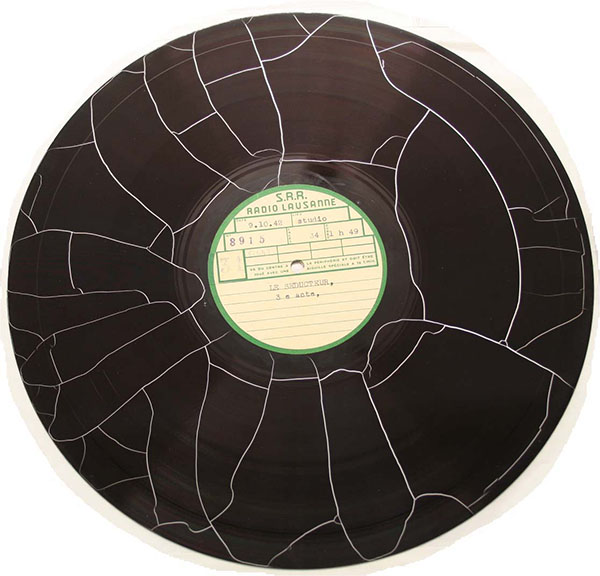
\includegraphics[width=0.7\textwidth]{images/cracked-disc}
\caption{An example of cracked disc.}
\label{fig:crackeddisc}
\end{figure}

Up to now, \gls{irene} and \gls{3dprobe} cannot automatically process such damaged records, because the groove traces are sometimes widely separated and may be shifted from each other. Though a special feature is implemented, enabling the user to manually track the traces, it is not a perfect tool for practical use. Moreover, even with such a feature, it could be really difficult to visually find the correct shifting when the traces look similar.

The aim of this Master's thesis is to find ways to read correctly these kinds of degraded records with the solutions developed at LBNL by Carl Haber and his team. In a first step, an improvement of the manual tracking will be implemented. It is still useful to keep it for some cases, e.g for special early recordings or when a disc is heavily cracked.

Then, the next step will be to design and implement a tracking feature able to process cracked records and link their traces automatically. VisualAudio already implements a feature enabling to track cracked discs in an automatic or semi-automatic way. It can then be taken as an example, though it will obviously not be possible to directly adopt its implementation, as the systems are quite different.

%\section{Report structure}

%TODO This report is separated in...

\chapter{Phonograph cylinders and records}

This chapter will give a quick historical overview of the different mechanical phonograph technologies and the types of mediums encountered. It will also explain the main principles behind the analog recording

\section{History}

The first known sound recording was realized by the French printer Édouard-Léon Scott de Martinville in 1860. However, the used device called the \emph{phonautograph} was not able to playback the recordings. It rather acted as an early oscilloscope and was used by scientists to study visual representations of the sound.

The phonograph was created by Thomas Edison in 1877. It was the first device able to record \emph{and} reproduce the sound. The general principle was to mechanically engrave the audio signal on a rotating cylinder. The resulting groove undulated then vertically. Then, for the playback, a stylus (needle) retraced the groove and was able to reproduce the sound waves from the generated vibrations. Finally, the signal was amplified with a horn so that the recording was audible. A newer version of this phonograph and an example of cylinder are presented in \autoref{fig:edisonphonocyl}.

\begin{figure}[!ht]
    \begin{subfigure}[b]{0.45\textwidth}
    \centering
    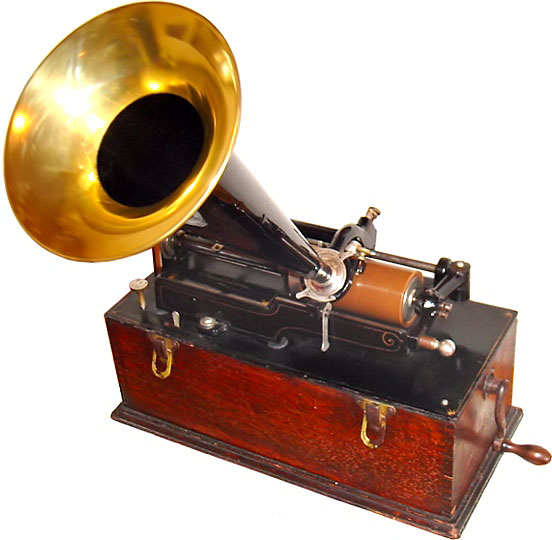
\includegraphics[width=0.8\textwidth]{images/edison-phonograph}
    \caption{An Edison phonograph.}
    \label{fig:edisonphono}
    \end{subfigure}
    \begin{subfigure}[b]{0.45\textwidth}
    \centering
    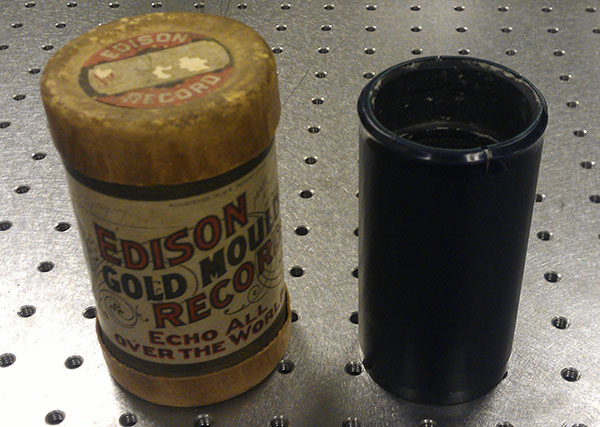
\includegraphics[width=0.9\textwidth]{images/edison-cylinder}
    \caption{An Edison wax-cylinder.}
    \label{fig:edisoncyl}
    \end{subfigure}
    \caption{Pictures of Edison wax phonograph and record.}
    \label{fig:edisonphonocyl}
    %\floatfoot{Norman Bruderhofer, www.cylinder.de}
\end{figure}

Since then, the phonograph has been used as the only device for sound reproduction until around the 1950's when the magnetic tape has become widely used on the market. From the first Edison's version, a lot of improvements have been made. Edison used first a tinfoil around the cylinders to engrave the groove. However, this material gave bad quality and was rapidly degrading. Alexander Graham Bell started to use wax-coated cylinders instead of the tinfoil, which improved a lot the sound quality.

Then, in the early twentieth century, the cylinders were gradually replaced by the gramophone records which were flat discs that could be double-sided. On the latter, the groove undulated laterally instead of vertically.

After the wax-cylinders, a lot of different materials have been used for the discs covering. For example, the shellac discs became the first widely used medium. Some discs were also using a special lacquer coat. Finally, the vinyl disc is one of the last types of gramophone record and is still being used today.

\section{Basic principle}

\subsection{Edison phonograph}

With the early Edison phonograph, the same device was used to record and play the sound. As already explained, the sound is mechanically engraved with a needle. In fact, the needle is connected to a diaphragm that vibrates when audio waves are emitted. The cylinder is put on a mechanism which can be rotated by a crank and that shifts slowly resulting in helical grooves, as represented in \autoref{fig:phonoschema}.

\begin{figure}[!ht]
\centering
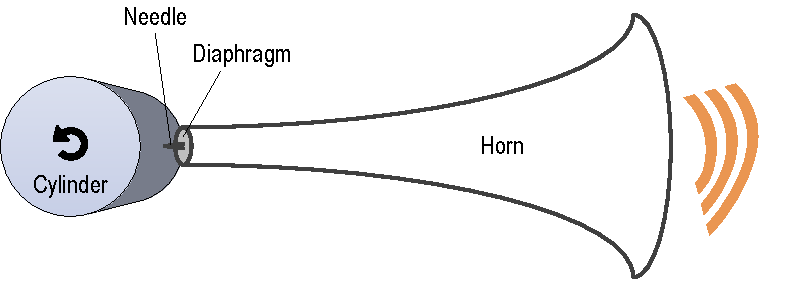
\includegraphics[width=0.9\textwidth]{images/phono-schema}
\caption{Schema of a simple phonograph.}
\label{fig:phonoschema}
\end{figure}

Then, to reproduce the recorded sound, the cylinder is repositioned at its starting position. The needle is placed with slightly less pressure, and when the crank is turned, the needle follows the groove which vibrates the diaphragm and returns the sound waves. This is in fact the exactly inverse process as the recording.

\subsection{Record types}
\label{sec:rectypes}

\subsubsection{Groove modulation}

The Edison phonograph uses a groove that undulates vertically. However, a lot of records, particularly the discs, have used laterally modulated grooves. This way, it is no more the depth that determines the signal, but rather the lateral position of the groove bottom. The difference can be clearly seen in \autoref{fig:groovesdiff}.

\begin{figure}[!ht]
    \begin{subfigure}[b]{0.49\textwidth}
    \centering
    
\includegraphics[width=0.8\textwidth]{images/grooves-vertical}
    \caption{Vertically modulated.}
    \label{fig:groovesvert}
    \end{subfigure}
    \begin{subfigure}[b]{0.49\textwidth}
    \centering
    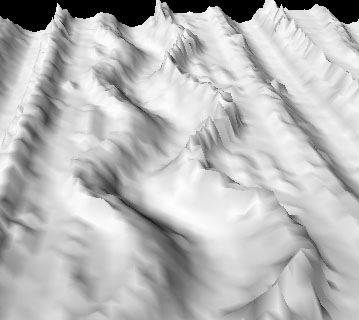
\includegraphics[width=0.8\textwidth]{images/grooves-lateral}
    \caption{Laterally modulated.}
    \label{fig:grooveslat}
    \end{subfigure}
    \caption{The two types of groove modulation.}
    \label{fig:groovesdiff}
\end{figure}

It exhibits a 3D representation of record surfaces for both groove types. In \autoref{fig:groovesvert} the boundaries are straight and the depth varies while in \autoref{fig:grooveslat} they form an horizontal wave.

\subsubsection{Revolution per minute}

Another important parameter is the number of revolutions per minute, abbreviated \emph{rpm}. It represents the rotational speed of the record while recording or playing. The speed of early records was not standardized, and it could vary from \SIrange[range-units=single]{60}{160}{rpm} for cylinders. Then, the speed has been progressively standardized to the common \SI{78}{rpm}. A lot of recording material to be restored now uses this format. The newer vinyl discs have then used the well-known speeds of \SI{33}{rpm} and \SI{45}{rpm}.

\section{Summary}

This chapter gave an idea of the phonograph history and different devices, showing the heterogeneous nature of the audio recording, with a lot of different techniques and materials. This outlines the difficulties that might appear while trying to recover old recordings.

The next chapter will discuss the technology developed at \gls{lbnl} in order to extract optically the sound from old records.

\chapter{Acquisition and processing systems}
\label{chap:acqprocsys}

This chapter details the systems used in the audio laboratory at \gls{lbnl} to extract records. For both systems, the main process is separated in two main steps: the acquisition and the processing.

\section{IRENE}

\subsection{Acquisition}

As already explained, \gls{irene} uses numerical macro photography for the acquisition. The scanner takes some monochromatic pictures of the disc. The resulting image is influenced by the shape of the surface because of the light reflection. Therefore, the intensity of the resulting pixels depends finally on the slope of the surface.

This enables to visually find the grooves on the resulting picture. An example of such a picture is shown in \autoref{fig:irenecapex}.

\begin{figure}[!ht]
\centering
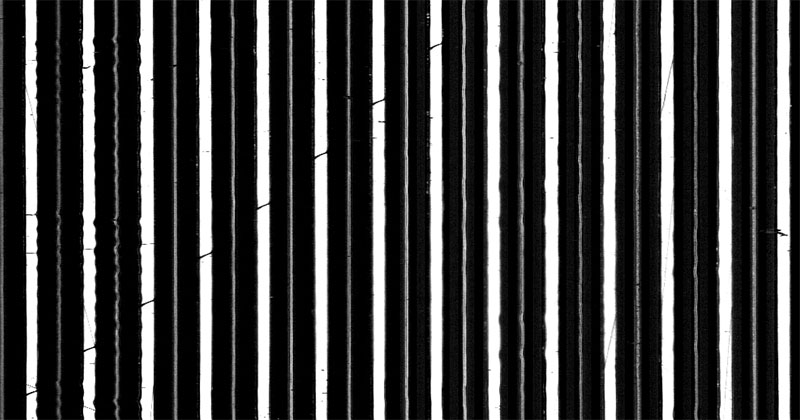
\includegraphics[width=0.7\textwidth]{images/irene-capture-ex}
\caption{IRENE capture excerpt.}
\label{fig:irenecapex}
\end{figure}

A single groove can be seen as two black strips with a thin bright line in between. The black parts represent the edges (higher slope) while the thin line is the bottom of the groove (very little slope, almost flat). Between two grooves, the structure is approximately flat, so the reflected color is also white. \autoref{fig:irenegroove} illustrates these different parts.

\begin{figure}[!ht]
\centering
    \begin{subfigure}[t]{0.29\textwidth}
    \centering
    \raisebox{0.3cm}{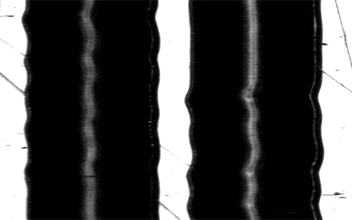
\includegraphics[width=4cm]{images/irene-grooves}}
    \caption{Two scanned grooves.}
    \label{fig:irenegrimg}
    \end{subfigure}
    \begin{subfigure}[t]{0.7\textwidth}
    \centering
    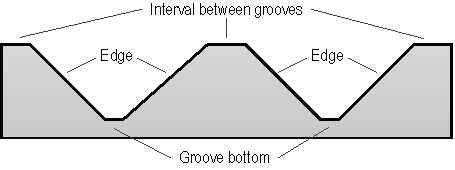
\includegraphics[width=9.5cm]{images/irene-grooves-schema}
    \caption{The corresponding shape.}
    \label{fig:irenegrschema}
    \end{subfigure}
    \caption{Visualization of scanned grooves.}
    \label{fig:irenegroove}
\end{figure}

\autoref{fig:irenegrimg} represents two grooves as they appear from the acquisition part. The approximate corresponding shape in a sectional view is visualized in \autoref{fig:irenegrschema}.

\subsubsection{Capture properties}

The camera cannot take a whole picture of one disc in a snapshot. It captures a line of \SI{3.072}{\milli\metre} with \num{4096} pixel samples. For a total disc revolution, \num{80000} lines are captured this way. Therefore, it results in an image of \SI[product-units=single]{4096x80000}{px} representing a ring-shaped disc capture in polar coordinates. To simplify the manipulation, the high resolution image is exported as eight separate pictures of \SI[product-units=single]{4096x10000}{px} easier to process.

For a \SI{78}{rpm} disc, the time for one revolution $t_{cyc}$ is the inverse of the rotational speed $w_{cyc}$. Therefore, the sampling rate $f_s$ for the system is given by
%
\begin{equation}
\label{eq:samprateirene}
f_s = \frac{n_{sample}}{t_{cyc}} = \frac{n_{sample}}{\frac{1}{\omega_{cyc}}} = \frac{\num{80000}}{\frac{1}{\SI{78}{rpm} \cdot \SI[quotient-mode=fraction]{1/60}{\metre\per\second}}} \approx \SI{104}{\kilo\hertz}
\end{equation}
%
This value satisfies the sampling theorem\footnote{The Nyquist–Shannon sampling theorem states that the minimum sampling frequency should be greater than twice the maximum of the sampled signal to reconstruct it properly. As the human hearing have a range from \SIrange[range-units=single]{20}{20000}{\hertz}, the sample rate for audio signal must be at least \SI{40}{\kilo\hertz}.} as it is greater than the minimum of \SI{40}{\kilo\hertz}.

\subsection{Processing}
\label{sec:processing}

After the acquisition, the original record is digitized and can be archived on digital media. To extract the sound, the next step is to use the \gls{rene} program. It offers features to process the record images and output the final corresponding sound as a \gls{wav} file.

\gls{rene} embeds a lot of algorithms and parameters to adapt at best the processing to the different record types. It is written in the \Csh{} programming language, enabling to easily build a complete graphical application without the use of third-party libraries. The \gls{gui} simplifies its utilization and offers the possibility to visually follow the tracking, as seen in \autoref{fig:irenegui}.

\begin{figure}[!ht]
\centering
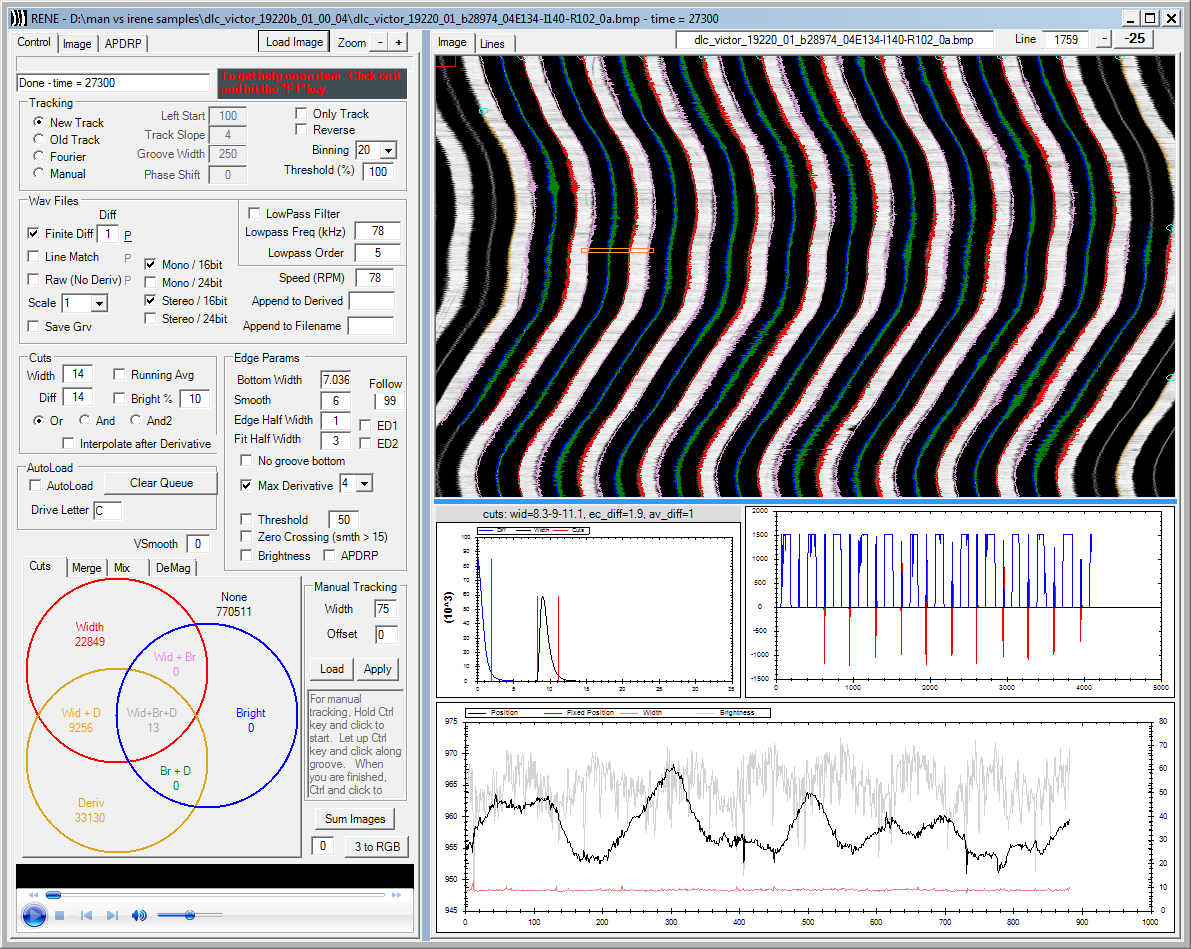
\includegraphics[width=0.9\textwidth]{images/rene-gui}
\caption{The IRENE user interface.}
\label{fig:irenegui}
\end{figure}

The left panel is used to specify the different parameters and algorithms for the separate steps and more generally to control the application. The upper right panel shows the processed record image. When the tracking is applied, the detected edge are directly drawn on top of the image. The panel at the bottom presents diverse information and statistics on the records.

The whole processing is applied in several steps.

\subsubsection{Tracking}

The tracking is a general groove detection algorithm. The image is binned in the vertical axis by a certain factor, resulting in a general view of the record. This is actually the view seen in the upper right panel (see \autoref{fig:irenegui}).

The tracking is applied on this binned image. This enables to approximately find the different groove positions, disregarding possible noise or imperfections cleared by the binning. The result of this step can be viewed on the top-panel in \autoref{fig:irenegui} as the purple and red external lines delimiting the grooves.

Several different algorithm can be selected to track the grooves. The best one to apply depends naturally on the scanned medium. As already mentioned, there is also an option to manually define the grooves position when the other methods are not applicable. The user can directly select points that define an interpolated line, which must follow the edge of the groove. This feature will be further explained in \autoref{sec:mancurrentimpl}.

\subsubsection{Image processing}

The next step is the actual processing. When the grooves are tracked, it remains to precisely find the groove center, which defines the sound information. Again, different algorithms can be used as methods using the derivative, thresholding, etc.

The result is the precise groove bottom defined between the blue and green traces on \autoref{fig:irenegui}.

\subsubsection{Sound processing}

Finally, it remains to create the output \gls{wav} file from the tracked groove bottom positions. At this step, some filters can also be applied to improve the sound quality.

\subsection{Architecture}

The diagram in \autoref{fig:renearchi} presents the general architecture of RENE.

\begin{figure}[!ht]
\centering
\includegraphics{diagrams/rene-gen-design.1}
\caption{General architecture of RENE.}
\label{fig:renearchi}
\end{figure}

The program does not use object-oriented design. The business logic and processing parts are embedded in the \texttt{Form1} class which also represents the view of the application (inheriting from the .NET WinForms \gls{api}).

Dependencies between the different classes are then fairly simple. Some tasks have been separated in external classes contained in the \texttt{Form1} class, as for the groove tracking or image processing which includes in fact routines to load images into bitmaps. The \texttt{DB} class handles connection and communication with a database, used to automatically store information and statistics on the processing results in a centralized database.

Some common processing tasks are separated in different utility classes, e.g. \gls{fft} algorithm or \gls{wav} processing to output the sound file.

\section{3D Probe}

\subsection{Acquisition}

With \gls{3dprobe}, the acquisition stage is the main difference. Instead of using a regular camera, a special probe is used, getting the actual depth for each point over a scanned part. This gives a real heightmap of the disc surface, as shown in three-dimensional view in \autoref{fig:groovesdiff}.

To measure the height of the scanned surface, the sensor takes advantage of the chromatic aberration \footnote{Optical distortion occurring when a lens cannot properly focus all colors of a same point due to different refractive indices for different wavelengths of the light.}. Light is emitted and passes through an objective. Because the refraction index depends on the wavelength, the light is refracted differently regarding the wavelength, as shown in \autoref{fig:chromaber}.

\begin{figure}[!ht]
\centering
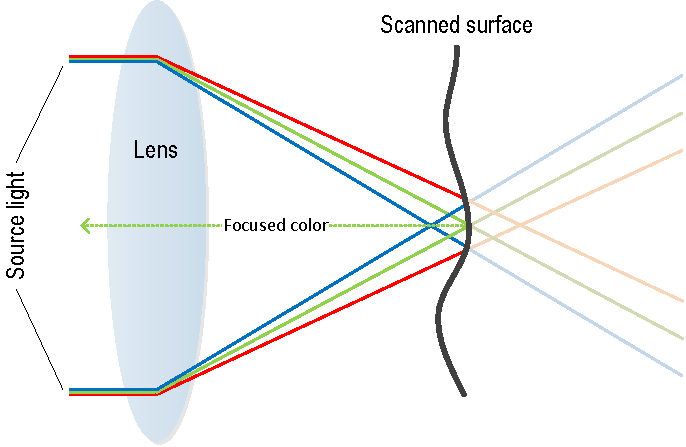
\includegraphics[width=0.8\textwidth]{images/chromatic-aberration}
\caption{Chromatic aberration through a lens.}
\label{fig:chromaber}
\end{figure}

Hence, the color reflecting in focus on the surface will depend on the distance from the lens. The sensor captures then the reflected wavelength and can deduce the height. The probe can also give the value of the brightness, that is, the captured light intensity for a given point.

\subsubsection{Capture properties}
\label{sec:captureprop}

In a single snapshot, the sensor is able to capture 180 points in one line of \SI{1.8}{\milli\metre} in a way similar to the 2D camera with \gls{irene}. The depth is measured in a range of \SI{400}{\micro\metre} with a resolution of \SI{0.125}{\micro\metre}.

The acquisition software outputs the data in a specific binary file format with extension \emph{.pri}, containing essentially floating-point values corresponding to the depth captures. The brightness is stored separately in a \emph{.bri} file, using exactly the same structure.

In this case, the number of samples for a full revolution depends on the angle $\alpha$ by witch the cylinder is rotated between two samples. Therefore, the sampling rate is not fixed and the formula for a cylinder at \SI{160}{rpm} become
%
\begin{equation}
\label{eq:samprate3d}
f_s = \frac{n_{sample}}{t_{cyc}} = \frac{n_{sample}}{\frac{1}{\omega_{cyc}}} = \frac{\frac{\ang{360}}{\alpha}}{\frac{1}{\SI{160}{rpm} \cdot \SI[quotient-mode=fraction]{1/60}{\metre\per\second}}}
\end{equation}
%

For example, with an angle $\alpha$ of \ang{0.02}, the number of samples is $\frac{\ang{360}}{\ang{0.02}} = \num{18000}$ and the sampling rate become $\frac{\num{18000} \cdot 160}{60} = \SI{48}{\kilo\hertz}$.

\subsubsection{Multiple-pass acquisition}

From the capture properties, the distance between two points is \SI{10}{\micro\metre}. The corresponding resolution is then quite low and could not be enough in some cases.

Therefore, the \gls{labview} acquisition software is able to perform a multiple-pass scanning. The same part a record is captured several times with a different shift. For example, by using two-pass, the number of points, and so the resolution are multiplied by two resulting in 360 points for the same distance.

\subsection{Processing}

The processing is done with the program called \gls{prism}. It uses the data stored in the \emph{.pri} and \emph{.bri} files to process and output the sound. The application is very similar to \gls{rene} and is also written in \Csh. There are also a lot of different parameters to tune the tracking and processing at best for the corresponding record type. Some parameters are also specifically related to cylinder processing.

The user interface (\autoref{fig:prismgui}) embeds approximately the same main parts as \gls{rene}, though differently disposed.

\begin{figure}[!ht]
\centering
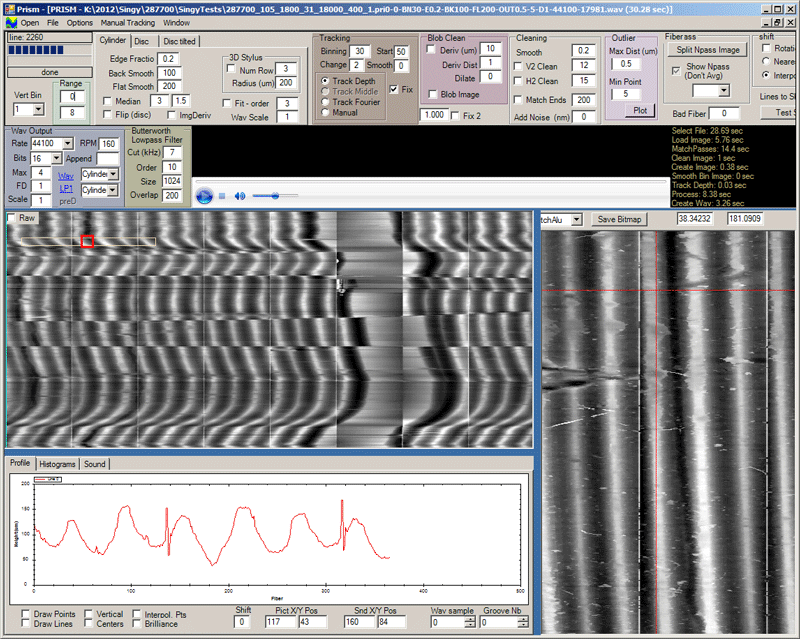
\includegraphics[width=0.9\textwidth]{images/prism-gui}
\caption{The PRISM user interface.}
\label{fig:prismgui}
\end{figure}

The parameters and algorithms can be set on the top panel. In the middle and the right, the scanned media is visualized as a 2D heightmap. The dark and bright colors emphasize the higher, respectively the lower points on the surface. The image at the left-hand side is a general view while the other one shows a full resolution portion of the record (selected with the cursor and highlighted with the red square on the left panel). The lower panel gives the same type of information as the other program.

\subsubsection{Processing steps}

The processing part is performed through the same steps as with \gls{rene} (see~\autoref{sec:processing}). The main point is to take into account that a pixel value now denotes a real height and no more a brightness difference as on a photography. Likewise, the 3D acquisition suffers from bad points, that is, pixels with incorrect height value coming from the acquisition. Special algorithms are then set up to clean the scanned data and suppress these bad points.

Finally, the cylinder processing algorithm is specific, as it considers of course the vertically engraved nature of these type of record (see~\autoref{sec:rectypes}). The waveform is indeed defined by the surface height in the groove bottom (the intensity in the heightmap) and not by its lateral position.

\subsection{Architecture}
\label{sec:prismarchi}

The general architecture of \gls{prism} is presented in \autoref{fig:prismarchi}.

\begin{figure}[!ht]
\centering
\includegraphics{diagrams/prism-gen-design.1}
\caption{General architecture of PRISM.}
\label{fig:prismarchi}
\end{figure}

The \gls{prism} program have a refined architecture, using more object-oriented facilities. The \gls{gui} is handled by the \texttt{frmMain} class. The big part of the business logic has been separated in its own class \texttt{Hardware}. This class represents an abstract record which is processed by the application. A inheritance hierarchy is built from it, mainly separated in \texttt{Cylinder} and \texttt{Disc} types representing vertically and laterally engraved records. This design enables to specialize the algorithms for any types of records.

Other utility classes handle common processing such as \gls{wav} creation or signal cleaning algorithms.

\section{Acquisition hardware}

Both \gls{irene} and \gls{3dprobe} use the same hardware for the acquisition. It consists of different sensors and motors connected to a controller. This controller is itself driven by a software, using a special library embedded in a \gls{labview} environment.

\subsection{Components}

There are two main different supports. The first one is a turntable specifically designed for flat discs with the scanner put vertically and the disc rotating horizontally. The second one enables cylinder scanning, the probe being placed horizontally and directly facing the record. \autoref{fig:labhw} represent the installation in the laboratory.

\begin{figure}[!ht]
    \begin{subfigure}[b]{0.49\textwidth}
    \centering
    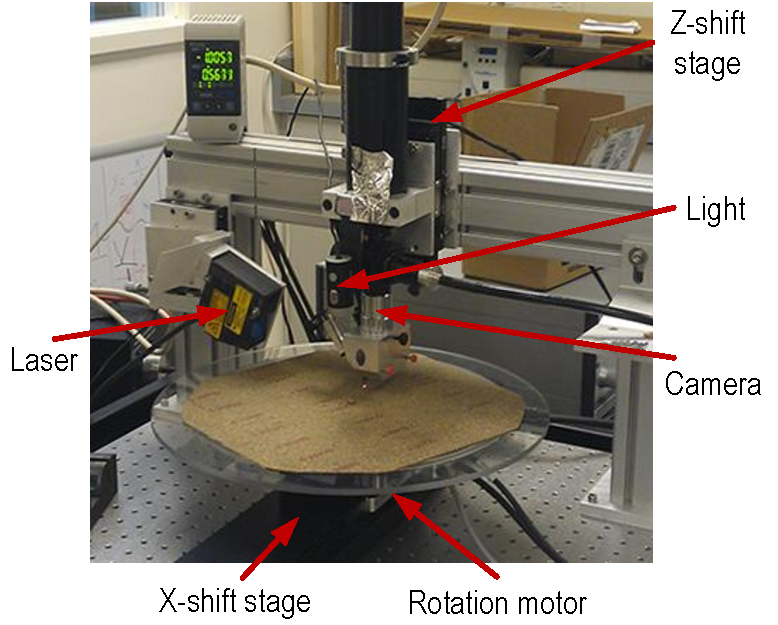
\includegraphics[width=\textwidth]{images/hardware-irene}
    \caption{The turntable to acquire flat discs.}
    \label{fig:labirene}
    \end{subfigure}
    \begin{subfigure}[b]{0.49\textwidth}
    \centering
    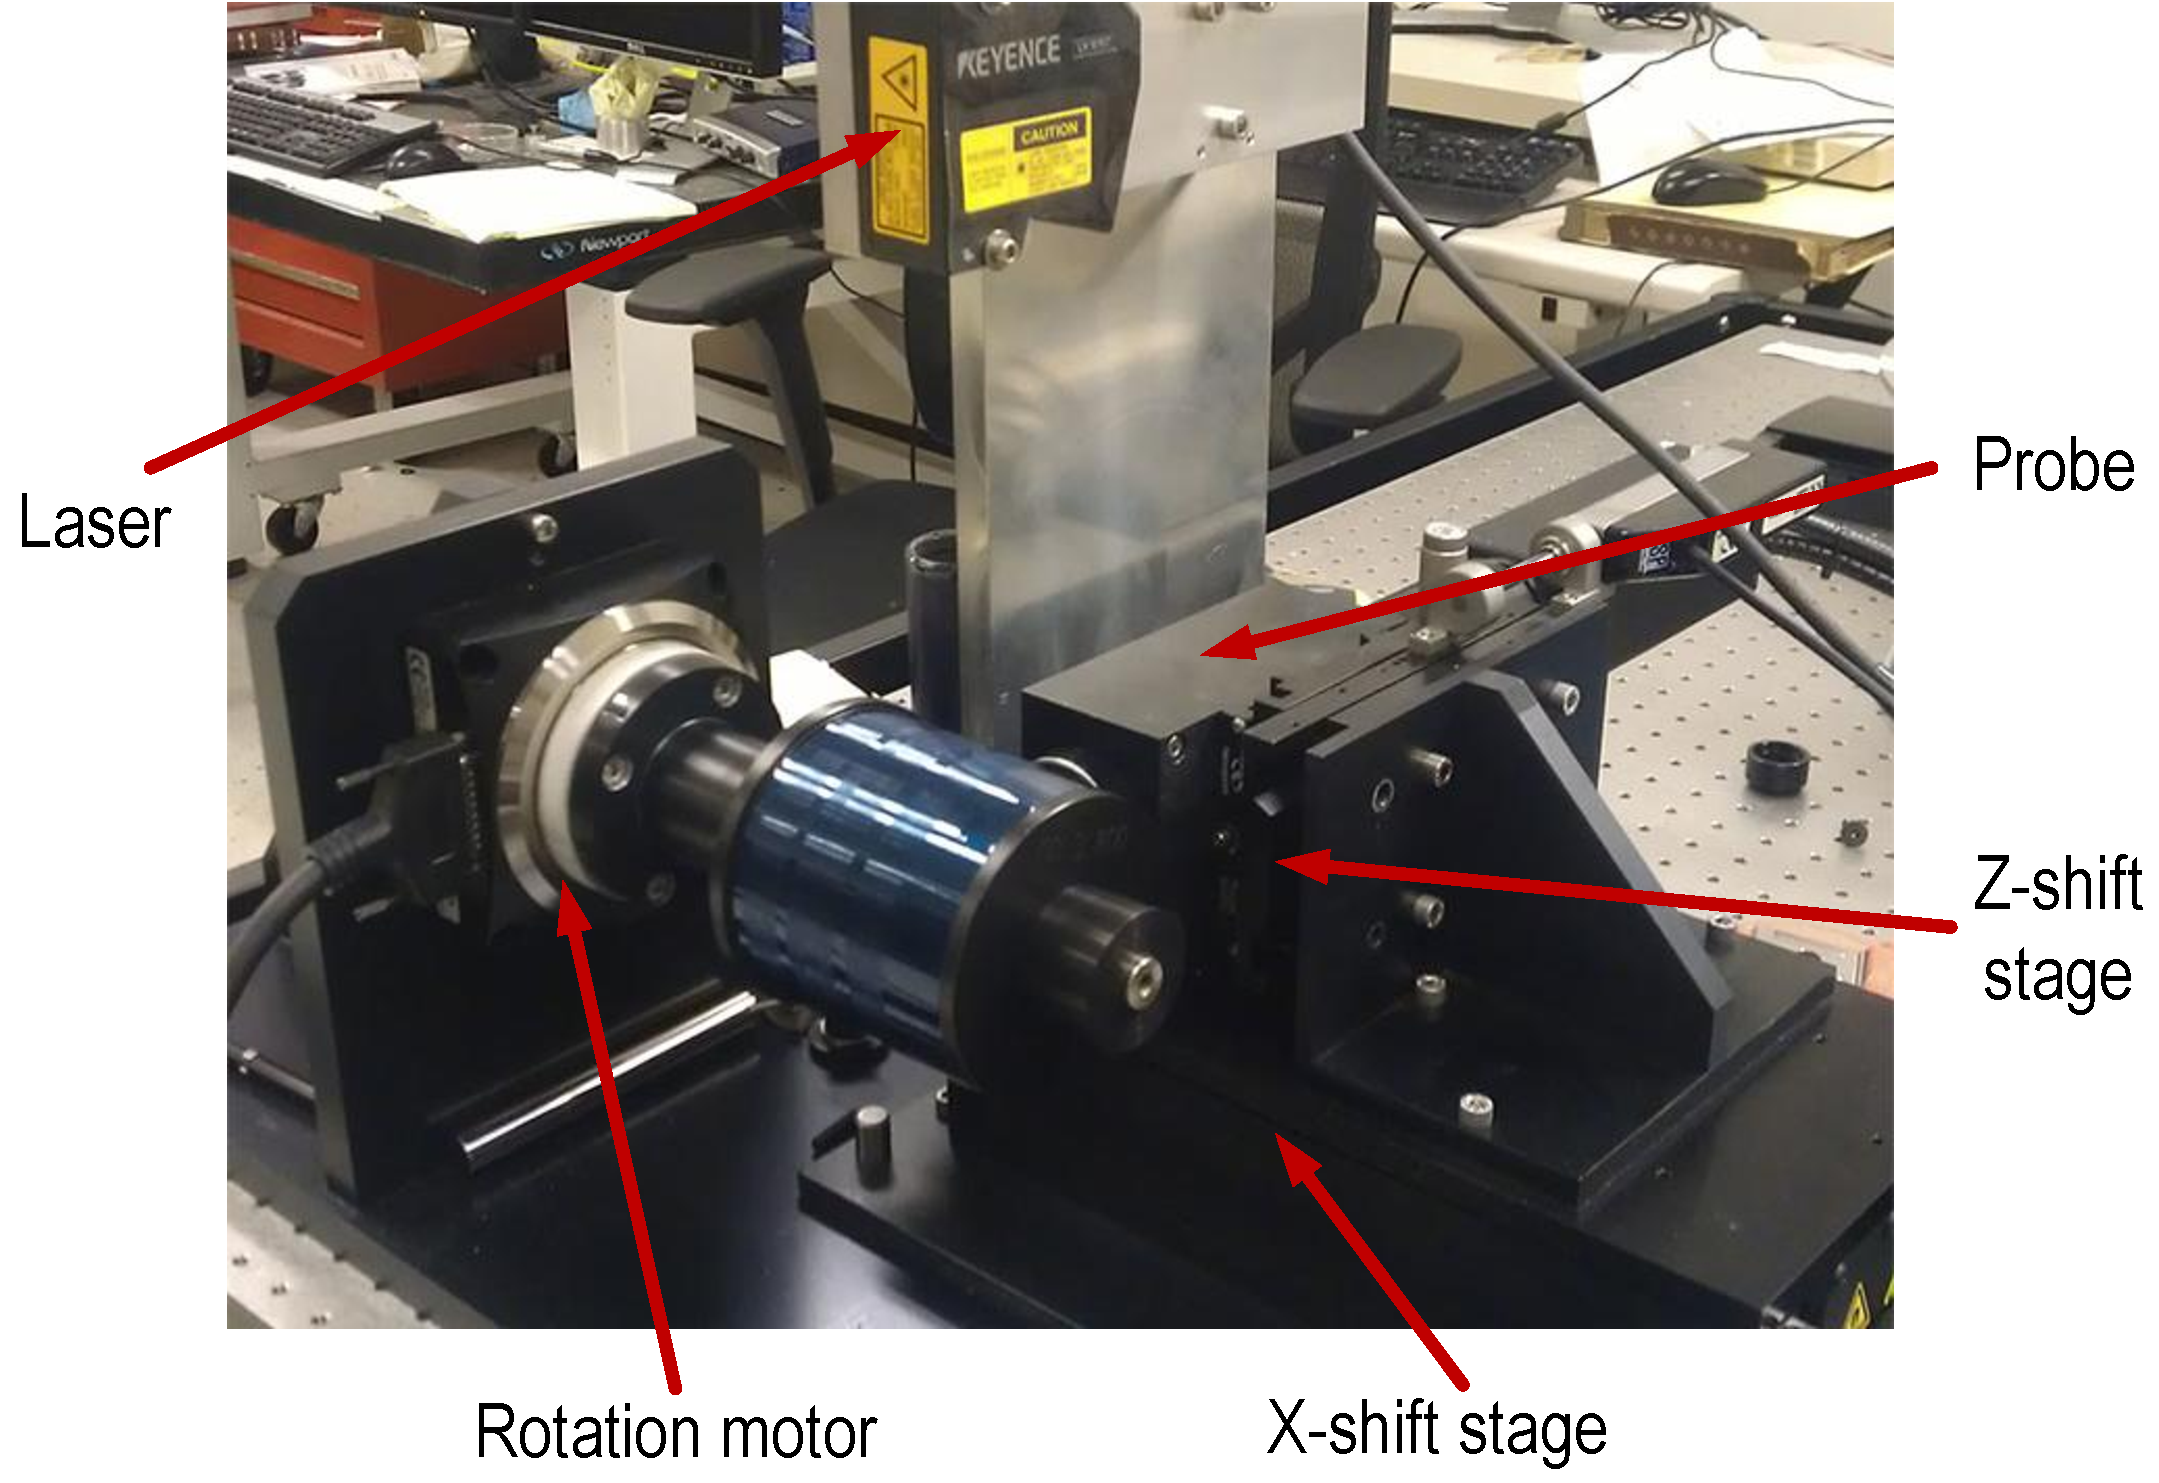
\includegraphics[width=\textwidth]{images/hardware-3d}
    \caption{The scanning equipment for cylinders.}
    \label{fig:lab3d}
    \end{subfigure}
    \caption{The acquisition hardware as installed at LBNL.}
    \label{fig:labhw}
\end{figure}

In both cases, in addition to the rotary motor, there is a X- and Z- shifting motor. The X-motor enables to shift the record to scan another portion. The Z-motor is used to adapt the sensor height for a correct focus.

\subsection{Z-correction}
\label{sec:zcorr}

Small differences can cause the 2D image to be blurred or the 3D scan to be out of range. To avoid this problem, a Z-shift correction is applied. The height shifting is controlled using a laser displacement sensor. It follows up the record and adjusts the sensor height, acting as an ``autofocus system''.

\section{Typical records issues}

As already stated, a lot of important and historical recordings are still stored on old records without other copies. Most of them can no more be read with regular phonographs. \gls{irene} and \gls{3dprobe} systems can then be used to restore the sound. However, some of the recordings are already altered, e.g. with some cracks appearing on disc surface, or completely broken into pieces, as old cylinders. These latter can still be acquired in several steps by strapping the pieces together, resulting in the same kind of issues in the processing step.

Depending on the degradation level, other issues can also appear with optical methods. In some cases they are still not able to perform a proper scan. The next sections depict the most common problems.

\subsection{Shifting}
\label{sec:issueshift}

Visible cracks on a record as shown in \autoref{fig:crackeddisc} is only the tip of the iceberg. Usually, it involves other problems to be solved algorithmically. One of the most common problem is shifting. When different parts of a disc surface are separated because of the cracks, they typically move slightly from each other, resulting in grooves mismatch. An example of this kind of issue is illustrated in \autoref{fig:shiftedgrooves}.

\begin{figure}[!ht]
\centering
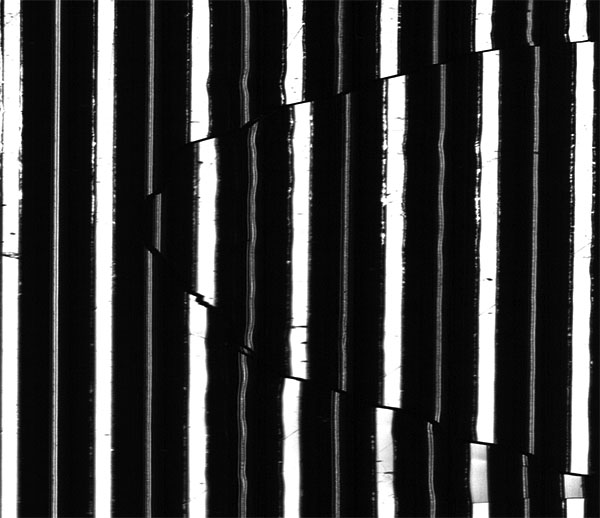
\includegraphics[width=0.6\textwidth]{images/shifted-grooves}
\caption{Grooves shifted because of a crack.}
\label{fig:shiftedgrooves}
\end{figure}

The acquisition shows clearly the two distinct pieces separated by a arch-shaped crack. In this case, the grooves are only slightly shifted. However the difference can be much larger and exceed up to several grooves large, causing difficulty to visually find the correct matching.

\subsection{Focus}

As explained in \autoref{sec:zcorr}, the acquisition needs always to stay in focus to get a sharp image. However, when the height varies abruptly, the laser is not able to directly compensate the Z-shift. This can happen sometimes when the lacquer inflates resulting in bubbles on the surface. The result in the acquisition is shown in \autoref{fig:blurredgrooves}.

\begin{figure}[!ht]
\centering
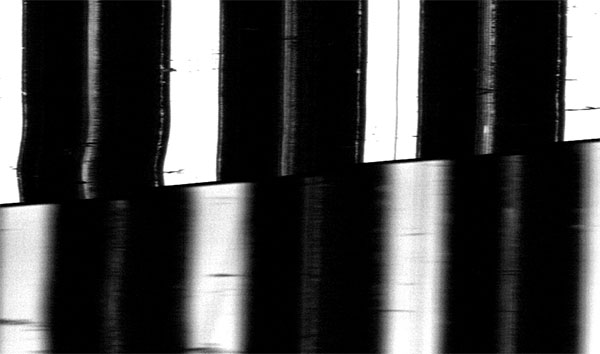
\includegraphics[width=0.6\textwidth]{images/blurred-grooves}
\caption{Blurred grooves on the bottom part under the crack.}
\label{fig:blurredgrooves}
\end{figure}

\subsection{Other issues}

Other problems may occur because of the cracks. For example, because of the lacquer deformation, the pieces can sometimes expand or shrink, which results in other corrections to apply. Likewise, the gaps introduced by the cracks can sometimes be large and the resulting sound affected. Most of time, the gap is not a loss of content but rather separation due to the shrinkage. Yet the reciprocal can also happen, i.e. when a piece of lacquer coat is folded on another one.

The trouble is to find out what is the best interpolation scheme to match the sound between the cracks. Furthermore, these latter issues become more important when a sound has to be synced with a visual representation, as for a movie sound track for example. The sound must match the picture so that the film is properly watchable.

\section{Summary}

This chapter presented an overview of the solutions developed at \gls{lbnl}. It covered the two systems, \gls{irene} and \gls{3dprobe}, both in terms of software and hardware. It also presented the common issues appearing while processing damaged audio records.

The next chapters will cover the existing ways of figuring out these issues, and the new implemented features during this thesis to improve it.

\chapter{Manual tracking}

This chapter explains how we improved the manual tracking. Because there are a lot of different mediums and the same amount of issues coming with, it is not likely to find the best solution to solve each of them. There are some recordings to be recovered that have particular and unique issues, appearing only in a small section of the record. Likewise, some small artifacts can appear visually easy to catch and fix for the human eye, but very tricky to solve with a particular algorithm.

Therefore, for this kind of thing, falling back to a manual tracking can be the more appropriate solution.

\section{Current implementation}
\label{sec:mancurrentimpl}

As summarized in \autoref{chap:acqprocsys}, both \gls{rene} and \gls{prism} feature similar manual groove tracking. The system is simple but useful on specific cases. To start tracking, the user must select the proper option in the tracking options. When clicking on the general record view with the CTRL key pressed (left image on \gls{prism}), a first tracking point is stored. Then, each successive click adds a new point and a polyline is drawn connecting all previous points, giving the general track path as seen in \autoref{fig:mantrackprism}.

\begin{figure}[!ht]
\centering
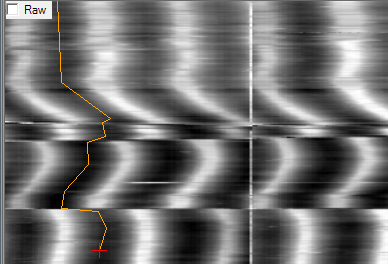
\includegraphics[width=0.5\textwidth]{images/manual-tracking-prism}
\caption{Manual tracking example in PRISM.}
\label{fig:mantrackprism}
\end{figure}

The program offers the possibility to store the tracked coordinates in a file to be used later. Finally, when the user applies the tracking, all points are interpolated and the processing step starts as usual.

\subsection{Limitations}

The current implementation is suitable to handle some complicated cases but suffers from several limitations:

\begin{itemize}
\item Unnatural way to draw a path over an image.
\item Tracking points can be manually put only on the binned (left) image, which can lack of precise information, especially if the scanned part is big and the record is cracked or damaged.
\item No possibility to undo parts already traced.
\item Tracking a whole record manually is a very slow process.
\end{itemize}

\subsection{Suggestions for improvement}

Regarding the previous limitations, several proposals were made at the project startup to find ways to improve the user experience and enhance the tracking efficiency.

\subsubsection{Touchscreen interface}

One of the concepts was to use a touchscreen interface. Nowadays, a lot of people are used to these interfaces such as tablets, smartphones, etc. Moreover, following a trace on a touch screen with the finger or a stylus seems to be user-friendly. This interface could also be convenient to re-align broken discs with shifted grooves (see \autoref{sec:issueshift}).

However, using a tablet would imply working on a specific operating system which would not be compatible with the current applications. It would be possible to implement a communication interface between the standard application and the UI but another problem could arise: these devices have mostly a limited capacity, while the amount of data processed for the sound recovery is very large. Nevertheless, using a simple touch screen within the current system and adapt the interface accordingly is still worth considering.

\subsubsection{Interactive tracking}
\label{sec:inttrack}

Another idea was to develop an \emph{interactive} way of tracking the grooves. The interface would display the groove scrolling \emph{continuously}, and the user would have to correct the lateral position to stay over the groove center.

The scrolling speed must be adaptable so that the tracking is convenient in different situations. Over areas where the surface is clean, it can be fast because there is no big correction to fix the track. When the right way is less obvious, the user can slow down and stop to choose the right way.

The zoom could also be adapted regarding of the speed. When the speed is slowed down, the zoom factor is greater to see precisely a specific part. When the speed is high, the user does not need to see the groove scrolling rapidly but should instead have an overview to stop at the next difficult point.

In fact, this feature could also be seen as a more entertaining way for this kind of work, because it could look like a ``game'' because of its animated and lively interface.

\subsubsection{Further improvements}

Beyond a brand new specific interface, other improvements to the user experience can be made to ease and accelerate the manual tracking.

The ability to undo what was done so far to be able to correct a wrong decision is a useful feature. Likewise, it could be gainful to be able to put some annotations before actually track the grooves. \gls{rene} and \gls{prism} already offer information and statistics about the scanned record. For example, one could notice that the signal on the graph between two shifted grooves is similar. It would then be possible to click on the specific ends to indicate that they are likely to be linked together for the tracking.

\subsection{Summary}

The current user interface for manual tracking is functional but can still be improved in many ways. The concept for a touchscreen interface is interesting but not easily applicable in the current state of the system. Therefore, the interactive method seems to be a good idea and its design and implementation is detailed in the next sections.

\section{Interactive tracking}

This section presents the interactive tracking feature as it has been integrated into the \gls{prism} program. The next subsections present it in terms of graphical interface, explain its utilization and detail its implementation.

\subsection{Graphical design}

\subsubsection{Location and integration}

As the current interface is already overflowed with all existing parameters and options, it is important to add the new feature so that it is integrated smoothly in the existing application, without making it tedious to use.

As seen in \autoref{fig:prismgui}, the interface is already able to show a detailed part of the disc on the right panel. When the user clicks on this detailed part, he can visualize other information on the signal. However, it is not designed to be interactive. In fact, each time the user selects a part on the right image, the corresponding part is reloaded and stored in a bitmap to be drawn on screen. The whole process is too time-consuming for an interactive drawing though it is suitable for its purpose.

The new feature has then to be separated from this detailed view. It has been chosen to put a tabbed panel to choose between the two configuration. As the user will not need both features at the same time, this is a suitable solution.

\subsubsection{Tracking panel}

The interactive tracking panel is separated in two parts: controls and visualization. The first part enables the user to manage and edit the different options while the second represents the record scan which the user has to follow to indicates the grooves. \autoref{fig:intpanelprism} represents the whole panel.

\begin{figure}[!ht]
\centering
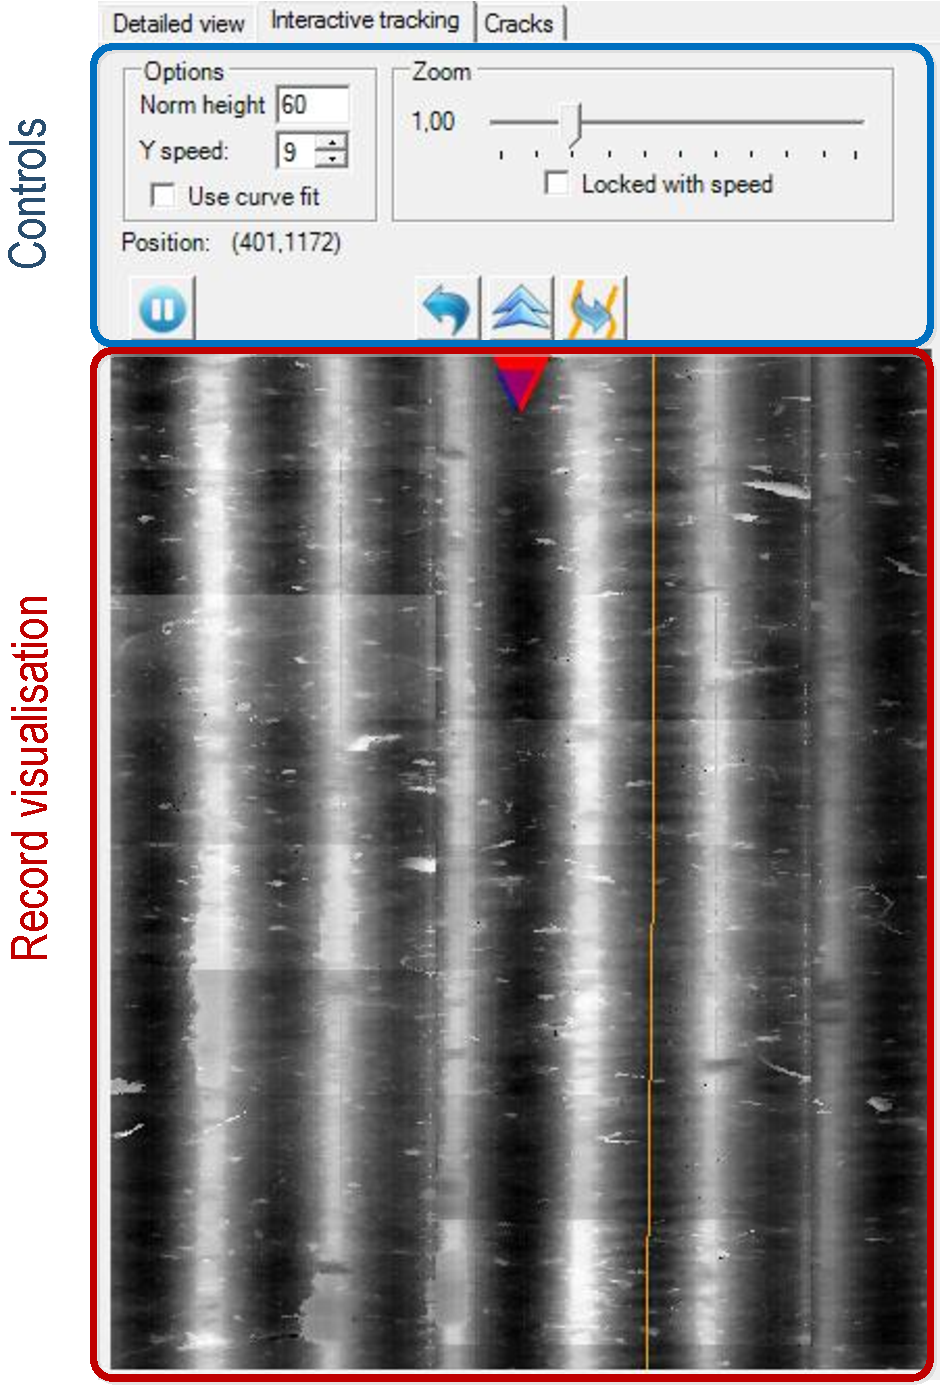
\includegraphics[width=0.6\textwidth]{images/int-track-panel-prism}
\caption{Interactive tracking panel in PRISM.}
\label{fig:intpanelprism}
\end{figure}

The controls enable to monitor the tracking by changing several parameters such as the speed or the zoom level. As explained in \autoref{sec:inttrack}, the zoom can also be locked regarding to the speed, using the corresponding option.

\subsection{Principle of operation}

To use the interactive tracking, the user first selects the corresponding button in the tracking options. Then, when the record is loaded, the corresponding disc is visible in the interactive panel. A red triangle acts as a beacon to clearly see the current tracked position.

When the user clicks on the panel and moves the cursor, the horizontal position moves accordingly. The goal is then to place the triangle tip on the center of the groove. While maintaining the mouse button pressed, the user may then increase the speed by using the mouse wheel. The record scrolls vertically while the horizontal position is still following the cursor.

To actually start the tracking, i.e. keep track of the points interpolated, the user must click the \emph{Play} button on the left.

\subsubsection{Synchronization between views}

The interactive view and the global view on the left are always synchronized. The current tracked position is visualized on the left panel of the application as a small red square and moves accordingly. When the tracking is performing, the corresponding polyline is drawn on the left part, as seen in \autoref{fig:intsynctrack}

\begin{figure}[!ht]
\centering
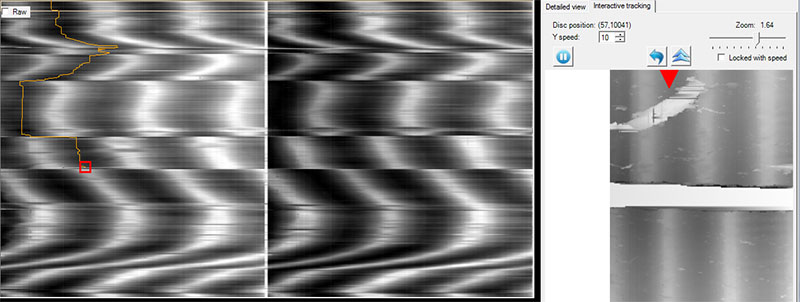
\includegraphics[width=0.9\textwidth]{images/int-track-sync}
\caption{Interactive tracking synchronized with the global view.}
\label{fig:intsynctrack}
\end{figure}

The reverse is also true. When the left panel is clicked, the position in the interactive panel is changed accordingly. When the tracking is running (the \emph{Play} button is pushed), a click on the panel also has the effect of adding an interpolation point. In fact, this acts in the same way as the original manual tracking. It is useful for some areas where the disc is in good quality and passing through the entire groove interactively would be too long. The user can easily switch between the two alternatives while tracking a record.

\subsubsection{Undo option}

One of the problems that happens with the manual tracking is the lack of an option to undo the last actions. It appears quite frequently that the last action is improper resulting in a bad tracking. The interactive tracking offers the possibility to undo the steps up to the starting point.

\subsection{Design and classes organization}

This part of the implementation is much about user interface and does not require a lot of processing. The main point is to find an appropriate way of integrating the new feature without blowing up the existing codebase which is already quite complex (see~\autoref{sec:prismarchi}).

The new feature has been implemented essentially in two new classes called \texttt{InteractiveControl} and \texttt{DrawPanel} as represented in the diagram of \autoref{fig:inttrackprismdiag}.

\begin{figure}[!ht]
\centering
\includegraphics{diagrams/int-track-prism.1}
\caption{Class diagram for the interactive tracking in PRISM.}
\label{fig:inttrackprismdiag}
\end{figure}

The first one embeds the whole control with the controlling part (toolbox) and the visualization path. It is a specific control and inherits the \texttt{UserControl} class of the WinForms \gls{api}. The specific interactive part drawing the record is handled by the second class. It inherits from the WinForms \texttt{Panel} class.

The interactive panel is owned by the \texttt{frmMain} class already created in PRISM. It uses the \texttt{Hardware} class for the communication with the record information, e.g. to get the original bitmap or set the points building the tracking path. The reference to \texttt{PictureBox} called \texttt{pict} and \texttt{picture} point to the same instance. It represents the left panel showing the global view. The \texttt{InteractiveControl} class needs it to force the drawing when the values are updated (e.g. while points are being added).

An utility class called \texttt{Utils} stands for common operations used specifically for the new feature.

\subsection{Implementation details}

%Though the this feature does not use a lot of processing code, different

\subsubsection{Bitmap creation}

At creation, the scanned record must firstly be converted to a bitmap, so that it can be drawn on the panel. Most part of the process is implemented in the \texttt{BitmapFromData()} in the utility class.

As already explained, the raw data of the scanned record is stored as an array of floating-point values (see~\autoref{sec:captureprop}). They must then be converted and normalized to be stored as values in the range \numrange[range-phrase=--]{0}{255} to represents pixel values. The bitmap created has the \SI{8}{bpp} format, using a 256 colors palette of grayscale values, so that the memory is not wasted with other colors.

\subsubsection{Draw panel animation}

The main implementation point is to update and draw the panel. This part is handled using \gls{gdi}, provided in Microsoft .NET through the \texttt{System.Drawing} classes.

As its name implies, \emph{interactive} means to draw the objects several times per second, so that it is possible to output a smooth animation. The way WinForms are usually handled is not meant to perform animation. The panels are refreshed only when required, e.g. when a window has been hidden by another, or when it is resized to replace the components. To refresh the panel manually, it must be marked as invalid by calling the \texttt{Invalidate()} function.

To perform an animation, one may then use a \texttt{Timer} (provided in the \gls{api}) and, at each tick, update the view before invalidating the panel. The interval should be set to a value giving a high enough refresh rate. For example, with an interval of \SI{40}{\milli\second}, the corresponding refresh rate is $1/0.04 = \SI{25}{fps}$.

\subsubsection{Linear transformations}

Another important consideration is the transformations. The stored information for the current position is, from an external point of view, the coordinates in the record where the red triangle is pointing. However, from the drawing area perspective, the triangle is fixed at the top center. Therefore, to draw the bitmap at the correct location, the drawing coordinates must then be inverted and shifted. When the target position is 30 pixels from the left and 200 from the top, the bitmap must in fact be translated by $(-30,-200)$. This is because they are two different coordinate systems involved, as viewed in \autoref{fig:inttracktransfo}.

Moreover, the zoom level influences the final position as well, and the final shift depends on this factor. Therefore, to handle easily the conversion, the best way is to alter the global transformation matrix before rendering the record bitmap instead of applying manually the transformations to the point. The corresponding code is presented in \autoref{lst:inttransfo}.

\begin{lstlisting}[language={[Sharp]C}, caption={Interactive panel drawing and coordinate systems transformation.}, label={lst:inttransfo}]
// In the painting function (g of type Graphics)a
Point renderPos = new Point(-position.X, -position.Y);

Matrix savedTransform = g.Transform;

// Coordinate system transformation
g.TranslateTransform(this.Width / 2, TRIANGLE_SIZE.Y);
g.ScaleTransform(zoomLevel, zoomLevel);

// Draw the record bitmap
g.DrawImage(bmpRecord, renderPos);

// Restore the transformation
g.Transform = savedTranssform;

// Draw the beacon triangle
int panelCenter = Width / 2;
g.TranslateTransform(panelCenter - TRIANGLE_SIZE.X / 2, 0);
g.FillPolygon(Brushes.Red, TRIANGLE_POINTS);
\end{lstlisting}

The initial transformation matrix is firstly saved. Then, when the bitmap has been drawn, it is reset to the normal one to draw correctly the triangle which is not influenced by the translation and scaling transformations.

One can note that the position is not inverted using a negative scale in the transformation, but is manually set by defining the \texttt{renderPos} variable. This is because if the bitmap is rendered with inversed scale, it will be drawn reversed, the bottom right coordinate becoming the top left one, which is not the desired behavior.

\begin{figure}[!ht]
\centering
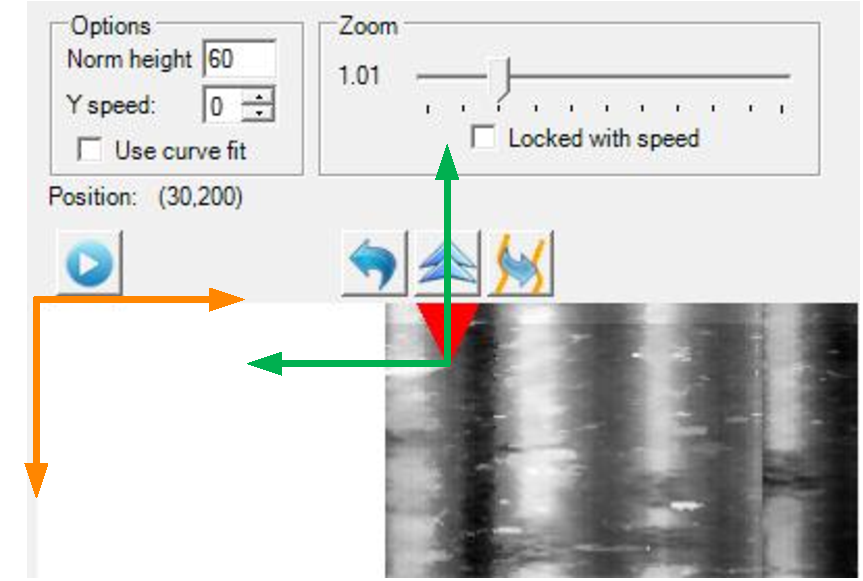
\includegraphics[width=0.6\textwidth]{images/int-track-transfo}
\caption[Coordinate systems in the interactive tracking panel.]{Coordinate systems in the interactive tracking panel. The drawing panel system is represented in orange and the record one in green. When the record is drawn at $(30,300)$, the bitmap is translated to the left and top.}
\label{fig:inttracktransfo}
\end{figure}

\subsection{Conclusion}

The new interactive tracking enables to simplify the sometimes painful manual tracking. It provides a new way to track the grooves and several enhancements helping the operator to restore records.

The next step will be to help finding the grooves by preprocessing the disc recording.

\section{Indicating grooves}

Another important thing, while manually tracking a record, is to be able to clearly find the groove bottoms. This seems not to be an issue as the groove bottoms are clearly seen in a lower intensity in \gls{prism} (and a lighter brightness with \gls{rene}). In fact, this becomes relevant when the disc are heavily cracked and separated into pieces. The main point is then to correctly match the pieces together, while the tracking inside a piece itself is easy to perform. The goal is to be able to bring out the groove bottoms at the bottom and top of all pieces, or chunks.

This feature is a bridge between a manual and an automatic solution. As it would be useful for the user to view this information, it will also be required for an automatic tracking system, to be able to reassemble them in a next step. The feature requires two big steps: find the groove bottoms and find the cracks.

\subsection{Finding groove bottoms}

A first step is to find the groove bottoms on a given Y-position. The usual tracking methods (see~\autoref{sec:trackprism}) do not need to find separate bottoms because once a groove is found, it can be followed until the end. This property is no more true on a damaged disc where the different parts can be shifted or even sometimes lost.

However, pointing out the position where the bottoms are located in an horizontal line is possible, using a adequate algorithm.

\subsubsection{Peak detection}

The values on an horizontal line on a record scan can be seen as a one-dimensional signal. To find the bottoms on a signal, one cannot use the simple mathematical derivative because the signal is too noisy. A lot of variation can happen between two different values, because the signal is not smooth as if given by a simple mathematical function. One must then use a peak detection algorithm.

Different algorithms exist. For example, one can just smooth the signal by averaging it (low-pass filter) and then use the zero-derivate method. However, a simple well-suited method that does not alter the original signal is presented in \cite{peak12}. The idea is to define peaks and valleys. In fact, a peak is a location where the values are the highest between two valleys. A delta value defines the minimum Y distance between a peak and the next valley.

\todo{Complete the section}

\section{Existing tracking methods}
\label{sec:trackprism}
\todo{Find a proper location for this section}

\subsection{Tracking depth}

One of the currently implemented automatic tracking method in \gls{prism}, called \emph{track depth}, tries to find the deepest point in a local region of the record. Then, it follows the corresponding X-position scanning the record downward and adjusting it to the deepest value. This method fails when their is just a little crack, because the depth is obviously completely wrong at these place, and the algorithm fails to find its way to the disc.

\subsection{Tracking Fourier}

TODO

%\chapter{Tests and extraction of the sample recordings}
%
%TODO.

%\chapter{Conclusion}
%
%TODO.

%------------------------ Float samples ------------------------

%\begin{figure}[!ht]
%\centering
%
\includegraphics[width=0.7\textwidth]{images/logo_lbnl}
%\caption{Image caption.}
%\label{fig:figname}
%\end{figure}

%\begin{table}[!ht]
%\begin{center}
%\begin{tabular}{| l c r |}
%    \hline
%    1 & 2 & 3 \\
%    4 & 5 & 6 \\
%    7 & 8 & 9 \\
%    \hline
%\end{center}
%\end{table}

%\begin{lstlisting}[language=C++, caption={Test listing}, label={lst:listingname}]
%// Comment
%int i;
%char c;
%\end{lstlisting}

%\autoref{eq:solve} with variable $s$ such as:
%\begin{equation} \label{eq:solve}
%s = [a_0, (a_0 + a_1), ..., (a_0 + a_1 + ... + a_{n-1})].
%\end{equation}

%\begin{figure}[!ht]
%\centering
%\begin{tikzpicture}
%\begin{axis}[xlabel=Hello 100 $x$,ylabel={$f(x) = x^2 - x + 4$},
%%height=5.2cm, width=\textwidth,
%]%xtick={0,0.5,...,20},]
%%xmin=0, xmax=2]
%%\addplot[domain=-10:10,color=blue,mark=*,mark size=1pt]{x^2 - x + 4};
%\addplot[domain=-10:10,color=blue,mark=*,samples=21]{x^2 - x + 4};
%\end{axis}
%\end{tikzpicture}
%\caption{Graph caption.}
%\label{fig:graphname}
%\end{figure}